%%%%%%%%%%%%%%%%%%%%%%%%%%%%%%
\chapter{Person Guidance}
\label{chapter:person_guidance}

The application of guiding a person to a location with a robot has many uses, such as giving tours in museums, showing a location to visitor and helping the visually impaired navigate. We think the guidance behavior is one of the most fundamental capabilities a socially interactive robot should have.

A straightforward approach to guide a person would be the the stop-and-wait method: robot plans a path and executes it normally as long as the guided person is nearby, and stops then the person is outside a defined radius. However, this method of guidance may lead to sudden stops and would not be socially accepted. A guide robot should consider the distance to the human and incorporate this information in its control strategy.

In this chapter, after reviewing the literature on guide robots in Section \ref{sec:guidance_related_work}, in Section \ref{sec:guidance_guide_robot} we present our guidance method, which adjusts the speed of the robot as a function of the distance to the person. Then we present a guidance in Section \ref{sec:guidance_blind_users}, specifically tailored for blind users.

\section{Related Work}
\label{sec:guidance_related_work}

The earliest works in guide robots focused on the implementation and long-term deployment of tour guide robots in public places such as museums. Burgard \cite{burgard1998interactive} presents the robot Rhino, that was deployed to a museum for $47$ hours. The Minerva robot was an improved model over Rhino \cite{thrun1999minerva}, and was deployed to a museum with an order of magnitude larger floor space. This robot was in operation for two weeks, and it was able to have short-term interaction with people via head motion and facial expressions. Siegwart \cite{siegwart2003robox} presents a robot that was deployed in an exhibition for 6 months. Nourbakhsh \cite{nourbakhsh2003mobot} presents a project where four guide robots were deployed to museums for a period of five years. The authors remark that it is indeed possible to deploy guide robots public places without supervision. All these tour-guide robots had various degrees of autonomy and was received with enthusiasm. However, in all of these works it was apparent that there is a need for research in the area of Human-Robot Interaction.

Pacchierotti \cite{pacchierotti2006design} demonstrates an office guide robot, but the main focus is on passing people in corridors. Clodic \cite{clodic2006rackham} presents another robot deployed in a museum. It was reported that a continuous interaction all along the guiding mission is fundamental to keep visitor's interest. Martin \cite{martin2004conception} studies the scenario of guiding a visitor in an office environment and focuses on robust person tracking. Pandey \cite{pandey2009step} focuses on the leave-taking of the guided person. The robot predicts the intent of the discontinuation of the task and either breaks the mission or searches for the user depending on the waiting time. Martinez-Garcia \cite{martinez2005crowding} focuses on the scenario of guiding a group of people with multiple robots at the same time. Garrell \cite{garrell2010local} works on a similar problem, where the task of the two robots is to control group of people and guide them. Another relevant scenario is the evacuation scenario, in which there is a danger and robots guide people to the safe a location \cite{kim2009portable,robinette2011incorporating}.

\section{Guide Robot}
\label{sec:guidance_guide_robot}

In this section, we describe how the guiding behavior is achieved. The robot's higher level actions are governed by a finite state machine, as shown in Figure~\ref{fig:fsm}. 

\begin{figure}[ht!]
\centering
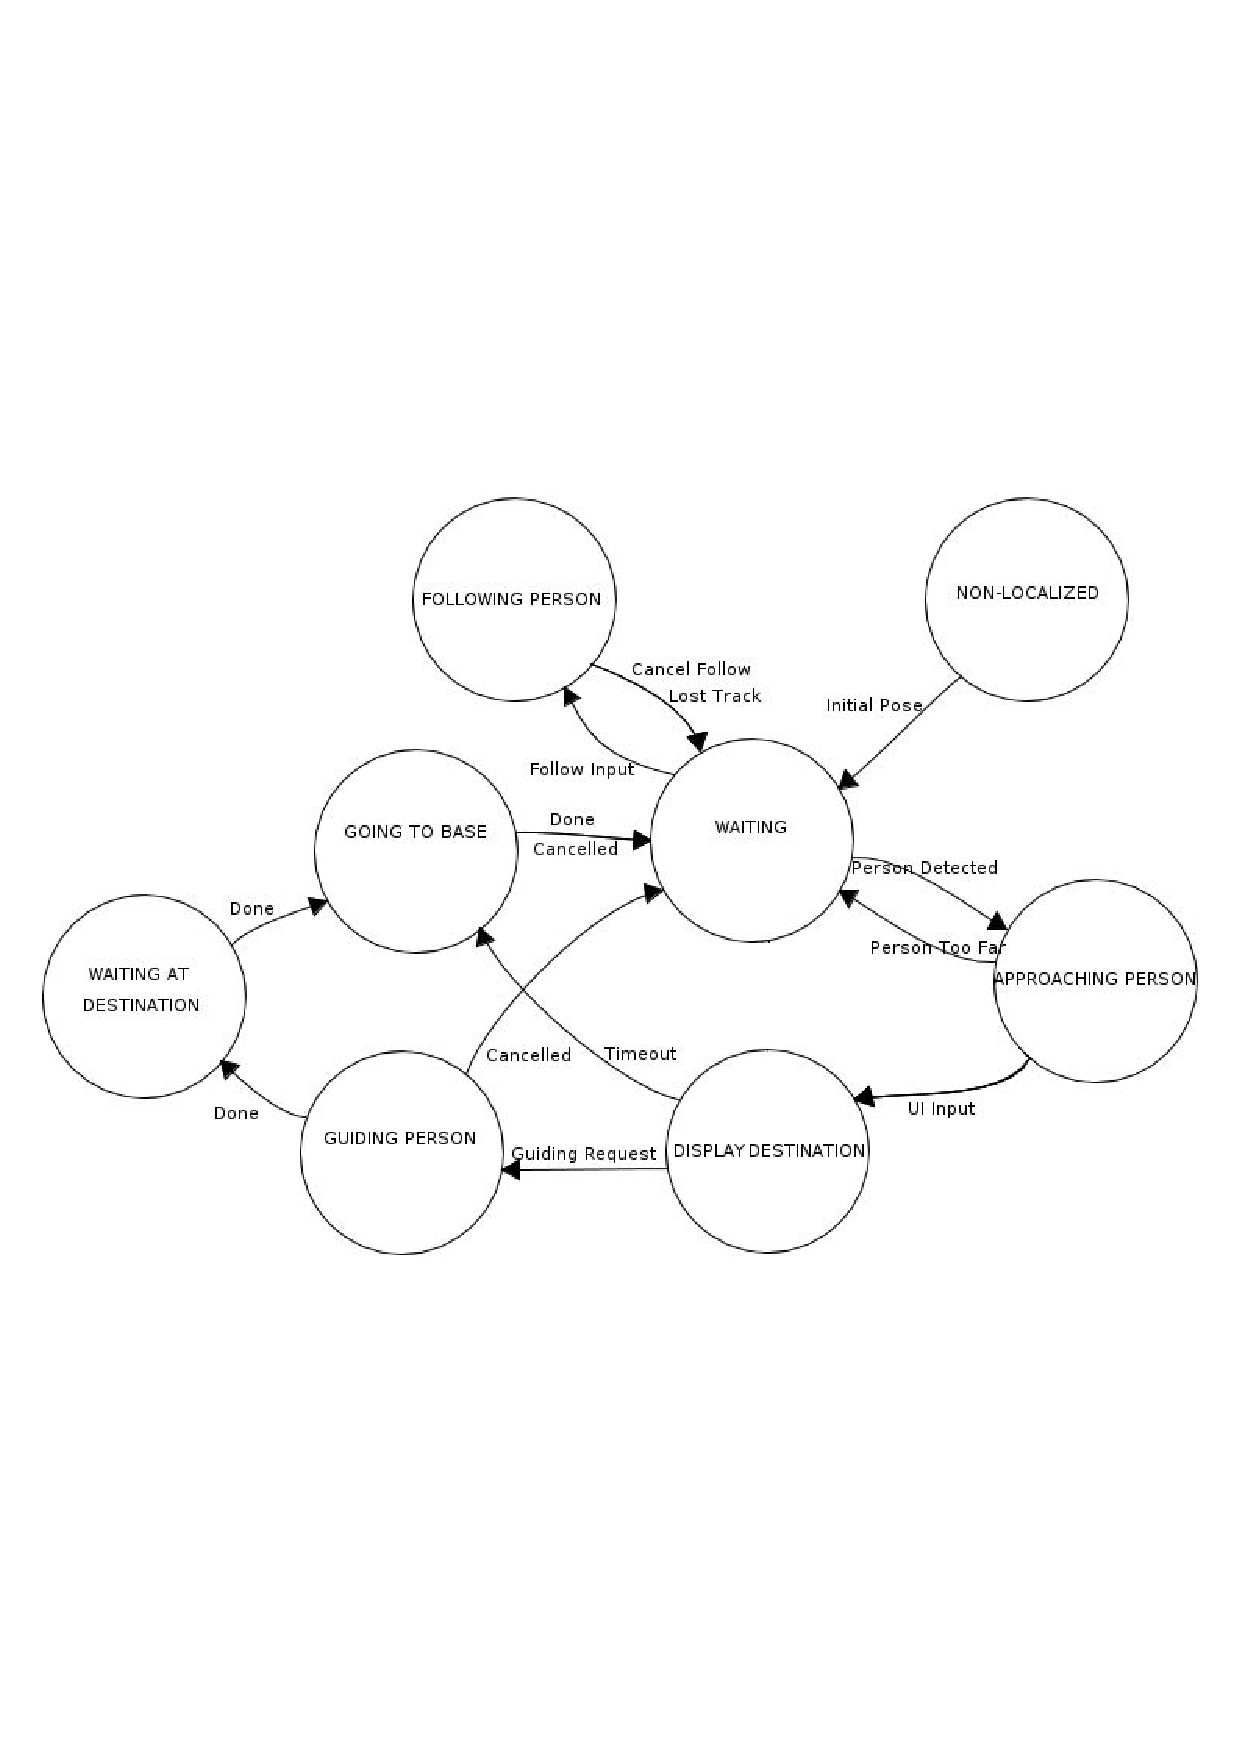
\includegraphics[width=1.0\textwidth]{pics/fsm}
\caption{Finite State Machine for the Guide Robot}
\label{fig:fsm}
\end{figure}

When the robot is started, it is in the \textit{NON-LOCALIZED} state. When the initial pose is given, either manually or by detection of the QR code (Section \ref{sec:mapping_localization}, robot switches to \textit{WAITING} state. This is the state where the robot actively looks input from users. When a person is closeby, robot approaches towards the person so the on-board tablet GUI is facing the potential user. If the person inputs a guide request, the robot displays destination and asks for confirmation. If the user confirms the goal, the robot is in \textit{GUIDING PERSON} state. When guiding is completed, robot waits for a while and goes back to the base. At any time, a user can cancel the operation or enter new commands.

After a request to guide a person is received from a higher level process, the robot first plans a path using a point-to-point navigation planner such as ROS Navigation or our navigation planner presented in Chapter \ref{chapter:navigation_among_people}. The robot continues on its path while constantly monitoring the distance between itself and the guided person, and adjusts its speed accordingly.


\begin{figure}[ht!]
\centering
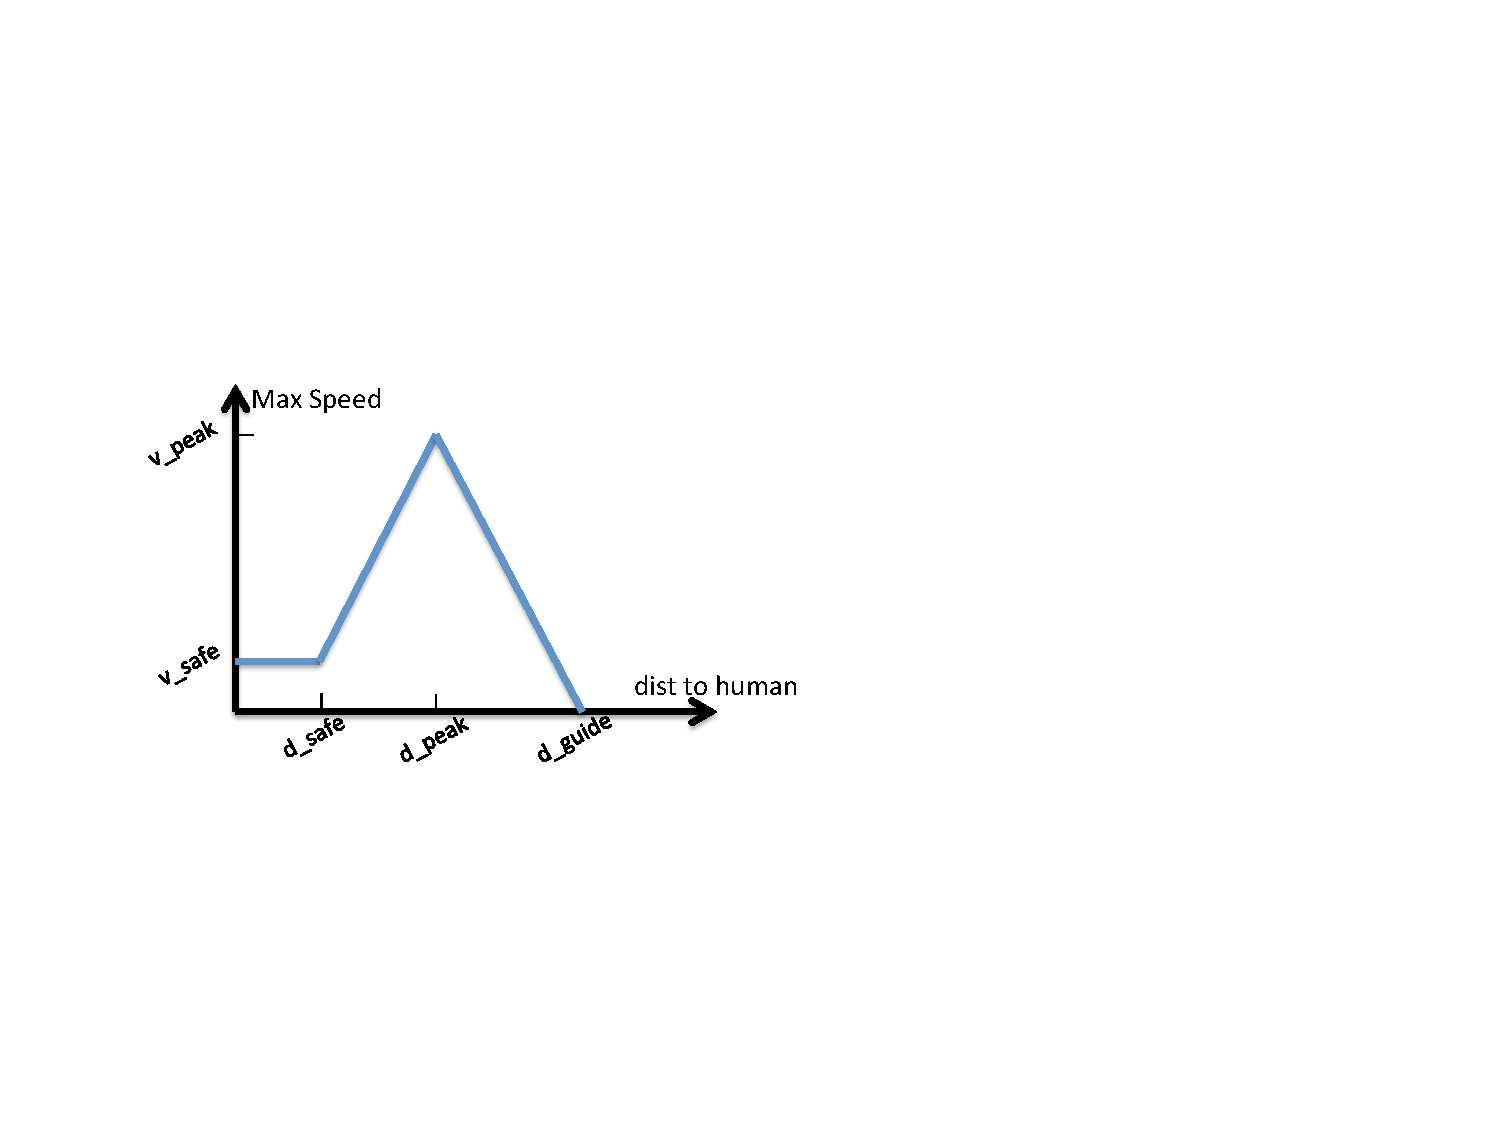
\includegraphics[width=0.5\textwidth]{pics/speed_profile_cropped}
\caption{Speed profile of a person guiding robot as a function of the distance to the user.}
\label{fig:guidance_speed_profile}
\end{figure}


We use a variable speed profile so that the robot can better keep up with the person and the motions of the robot is smoother. We define a speed function that is a function of the distance between the robot and the user. This speed profile is shown in Figure \ref{fig:guidance_speed_profile}. The robot moves at a low speed $v_{safe}$ if the human is dangerously close. The speed is peaked at distance $d_{peak}$ and the robot stops if the distance is larger than $d_{guide}$, which may indicate that the human is not interested in being guided. Note that $v_{peak}$ is capped by the speed limits in the environment, provided by the speed map approach presented in Section \ref{sec:navigation_speed_limits}.

\subsection{Pilot Study}

We evaluate the proposed guidance method in a comparison study. The task of the robot is to guide a person in an office environment. Figure \ref{fig:nav_speed_map_corridor} shows the part of the map and the goal of the robot. There are not any other people in the environment other than the guided person and ROS Navigation is used for point-to-point navigation planning. The robot actively guides a user to this goal position, in the following two conditions:

\begin{enumerate}
\item Stop-and-wait: The robot stops as long as the distance to the user is higher than a threshold
\item Proposed method: The maximum speed of the robot is altered as a function of the distance to the user. The velocity profile shown in Figure~\ref{fig:guidance_performance_graph} is used with $d_{guide}=1.7$m, $d_{peak}=0.9$m, $d_{safe}=0.1$m, $v_{safe}=0.1$m/s, $v_{peak}=1.0$m/s.
\end{enumerate}

In the experiment, when guiding was enabled, the human first waited until the robot stopped at $d_{guide}$. Then he took a step and waited for a second time, and then started following the robot. We track the position of the human with our torso tracking approach. As evaluation metrics, we measure the instantaneous speeds of the robot and the human.

\subsection{Results}
\label{sec:guidance_results}

The comparison of robot speeds is given in Figure \ref{fig:guidance_graph_noadj} for Condition 1 and Figure \ref{fig:guidance_graph_adj} for Condition 2. Between $t=0$ and $t=9s$, the accelerations were higher for the stop-and-wait condition. Robots that exhibit high accelerations will likely be perceived as unsafe, therefore the proposed method exhibits more socially acceptable behavior. Moreover, after the person started closely following the robot ($t >9s$), our approach is better at mimicking the speed of the human.

\begin{figure}[ht!]
\centering
%
        \subfigure[]{%
        	\label{fig:guidance_graph_noadj}
            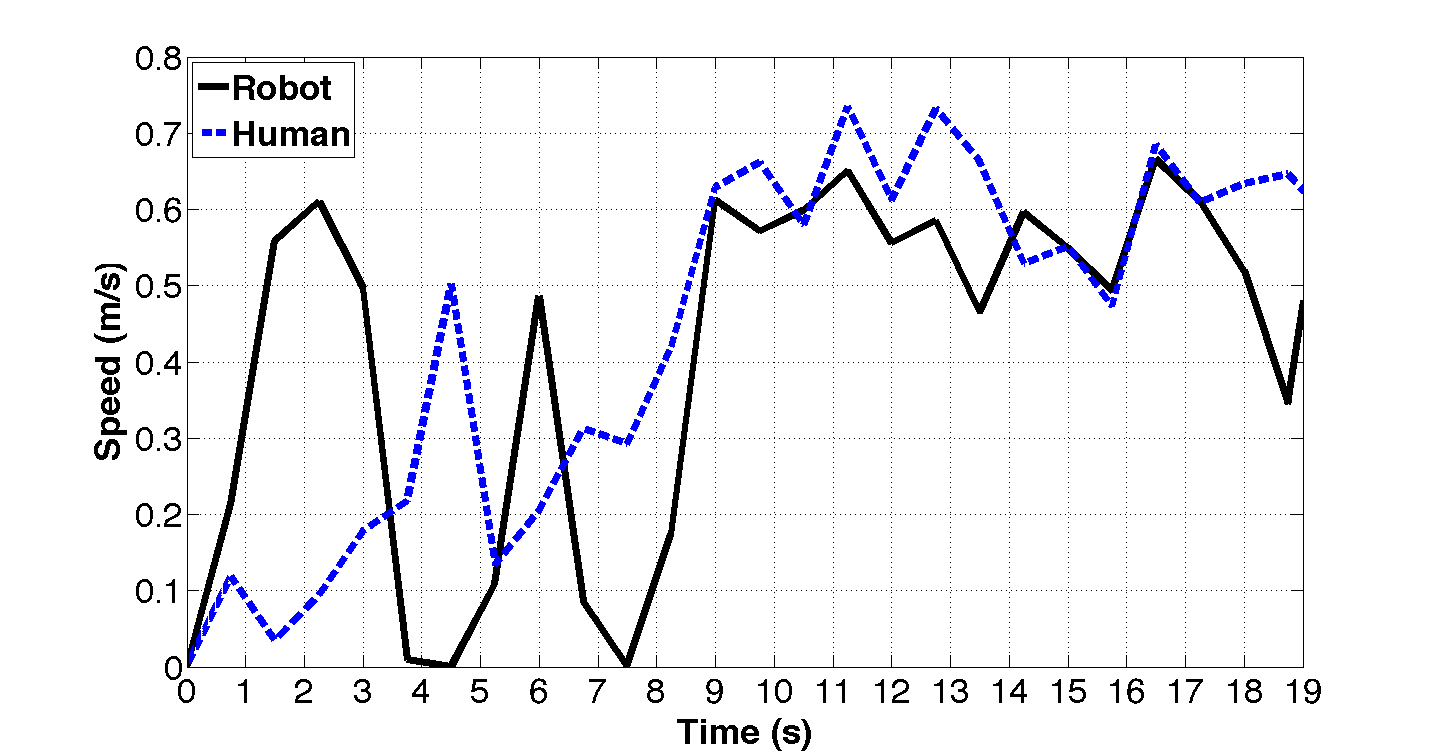
\includegraphics[width=0.75\textwidth]{pics/graph_noadj}
        }%\\
        
        \subfigure[]{%           
                	\label{fig:guidance_graph_adj}
           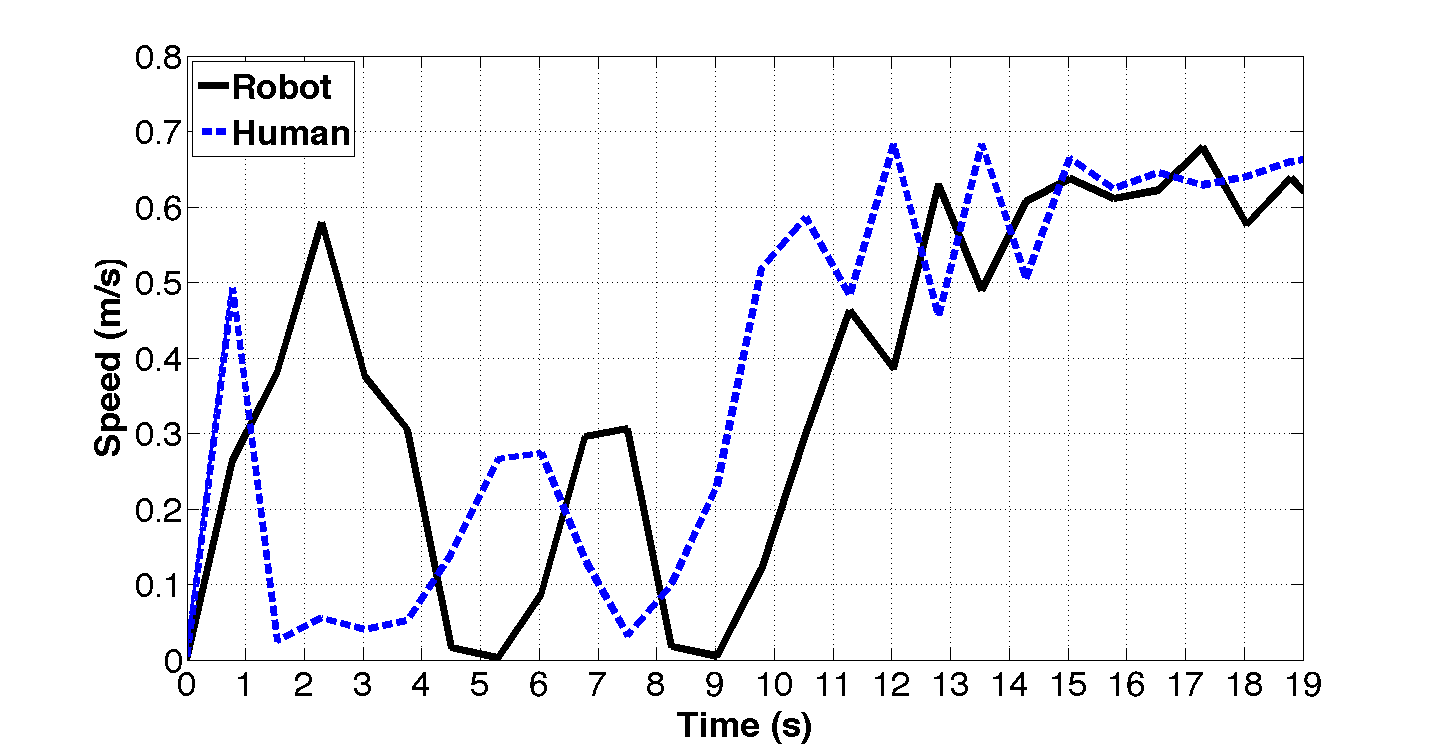
\includegraphics[width=0.75\textwidth]{pics/graph_adj}
        }        
    \caption{%
	Comparison of robot and human speeds are shown for two person guidance methods. a) Stop-and-wait guidance with ROS Navigation b) Proposed guidance method. Accelerations were less steeper in b).
     }%
   \label{fig:guidance_performance_graph}
\end{figure}




\section{Application To Blind Users}
\label{sec:guidance_blind_users}

In this section, we present our person guidance system specifically tailored for guiding blind users. Our approach consists of planning a path for the user and applying vibrations via a haptic belt to keep the user on the path.

%System graph, persception ellipse

\subsection{Tactile Belt}

In the previous section, we assumed that the guided person can detect where the robot is. With a blind user, this assumption does not hold. Therefore we need a mechanism to give directions to the user. Readily available options for assistive interfaces are limited to Braille or devices that presents content with speech synthesis. These ways of presenting information have difficulty dealing with representing spatial information. We also think visually impaired individuals would prefer a non-speech interface because they mostly rely on their sense of hearing in daily life. We therefore use a tactile belt for navigation guidance, because it can represent directions and rotations, be worn discreetly and does not occupy the hearing sense.

The belt has 8 pancake vibration motors, linearly spaced around the waist, and the motors can be controlled asynchronously via an Arduino board. We used two distinct vibration patterns to control the person's movements:

\begin{enumerate}
\item Directional Movement: When the guided person should move in a direction
\item Rotational Movement: When the guided person should turn around self
\end{enumerate}

The vibration patterns that induce directional and rotational movements in the human can be specified in many ways. We evaluated four patterns in each category with a user study. The details of this user study as well as a survey about the usability of the Tactile Belt is provided in Appendix \ref{chapter:vibration_pattern_analysis_for_haptic_belts}. The user study showed that the directional motion pattern with the highest recognition rate and least reaction time was the \textbf{TWO TAPS} pattern, which is illustrated in Figure \ref{fig:vibration_pattern_two_taps}. For the rotational motion pattern, we used the continuous rotation with a single motor, illustrated in Figure \ref{fig:vibration_pattern_solo_cont}. 

\begin{figure}[ht!]
\centering
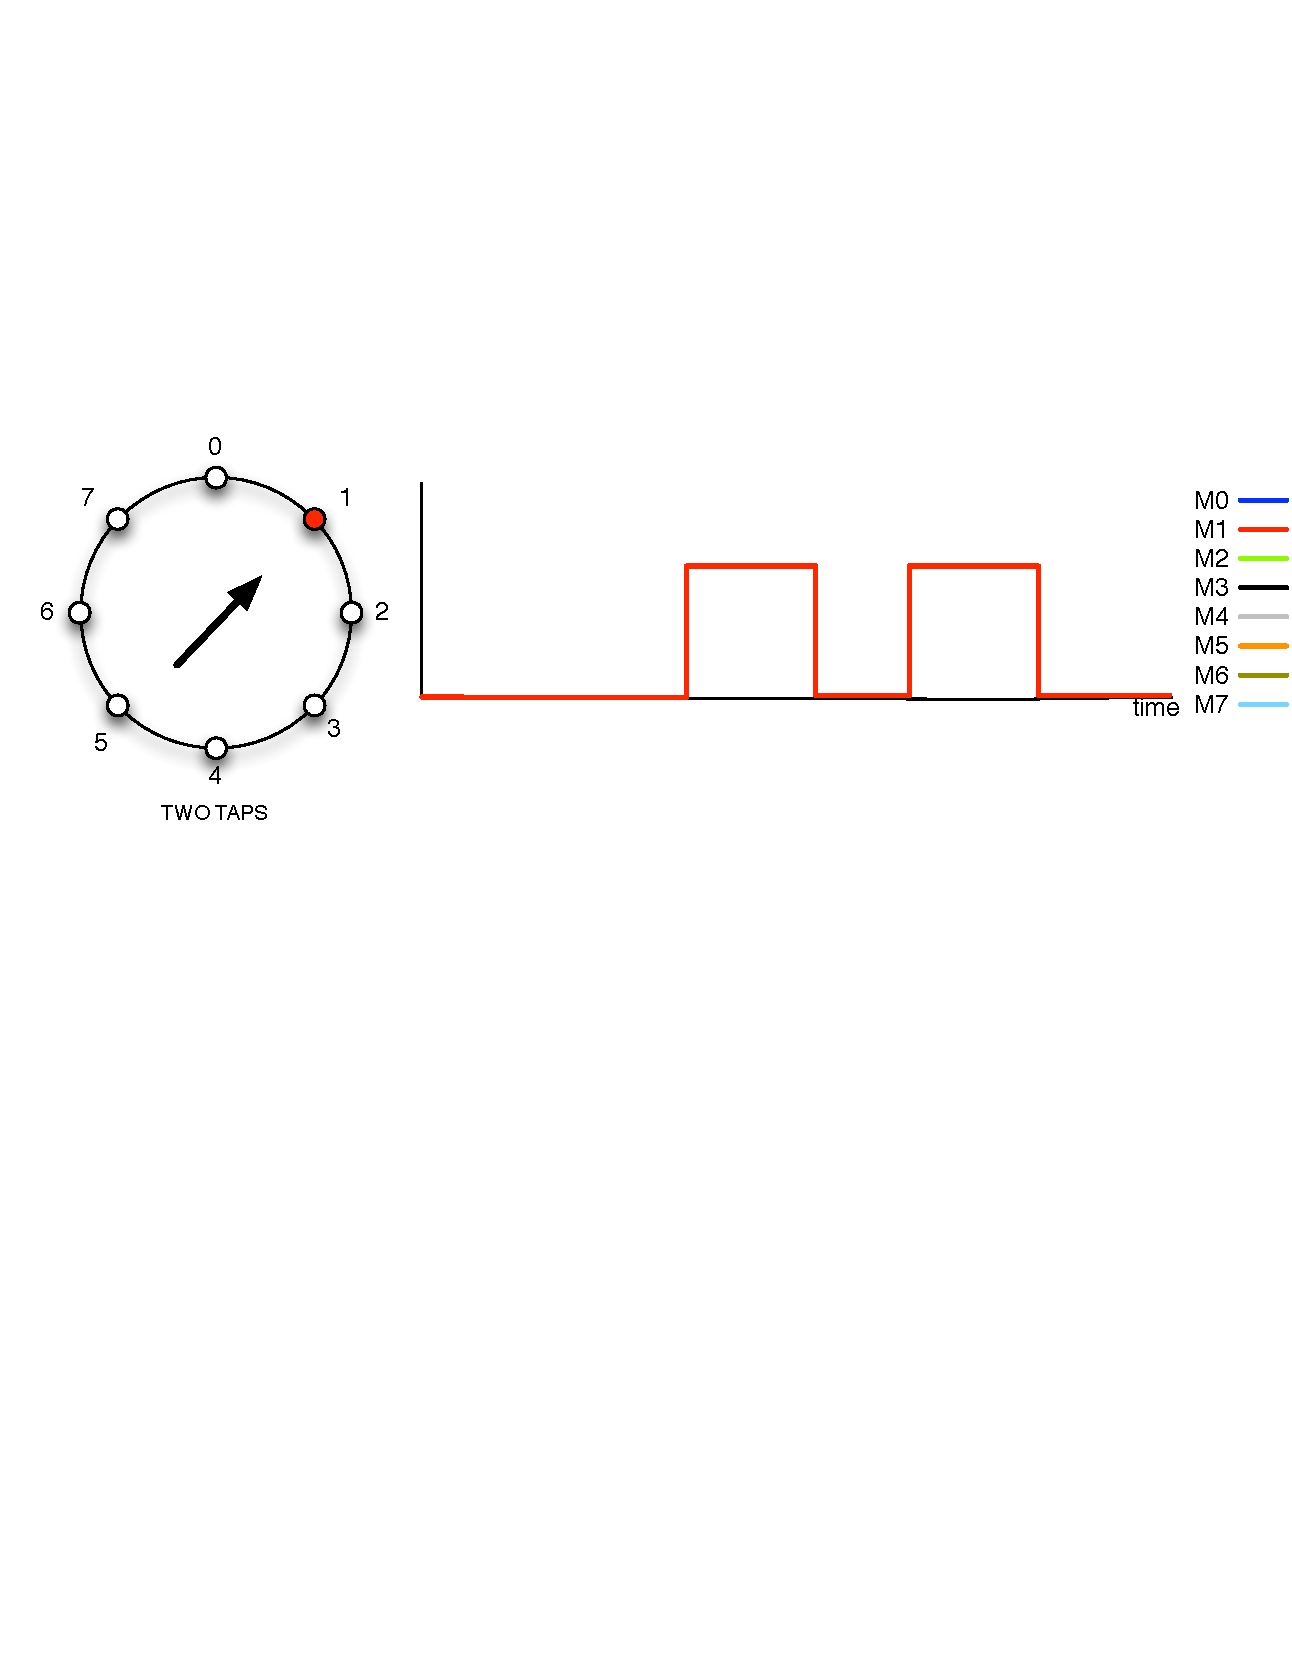
\includegraphics[width=1.0\textwidth]{pics/vibration_pattern_two_taps}
\caption{The vibration pattern applied by the Tactile Belt to induce directional movements in the blind user. A motor is fired for a duration of $250ms$, inactivated for $250ms$ and fired again for $250ms$.}
\label{fig:vibration_pattern_two_taps}
\end{figure}

\begin{figure}[ht!]
\centering
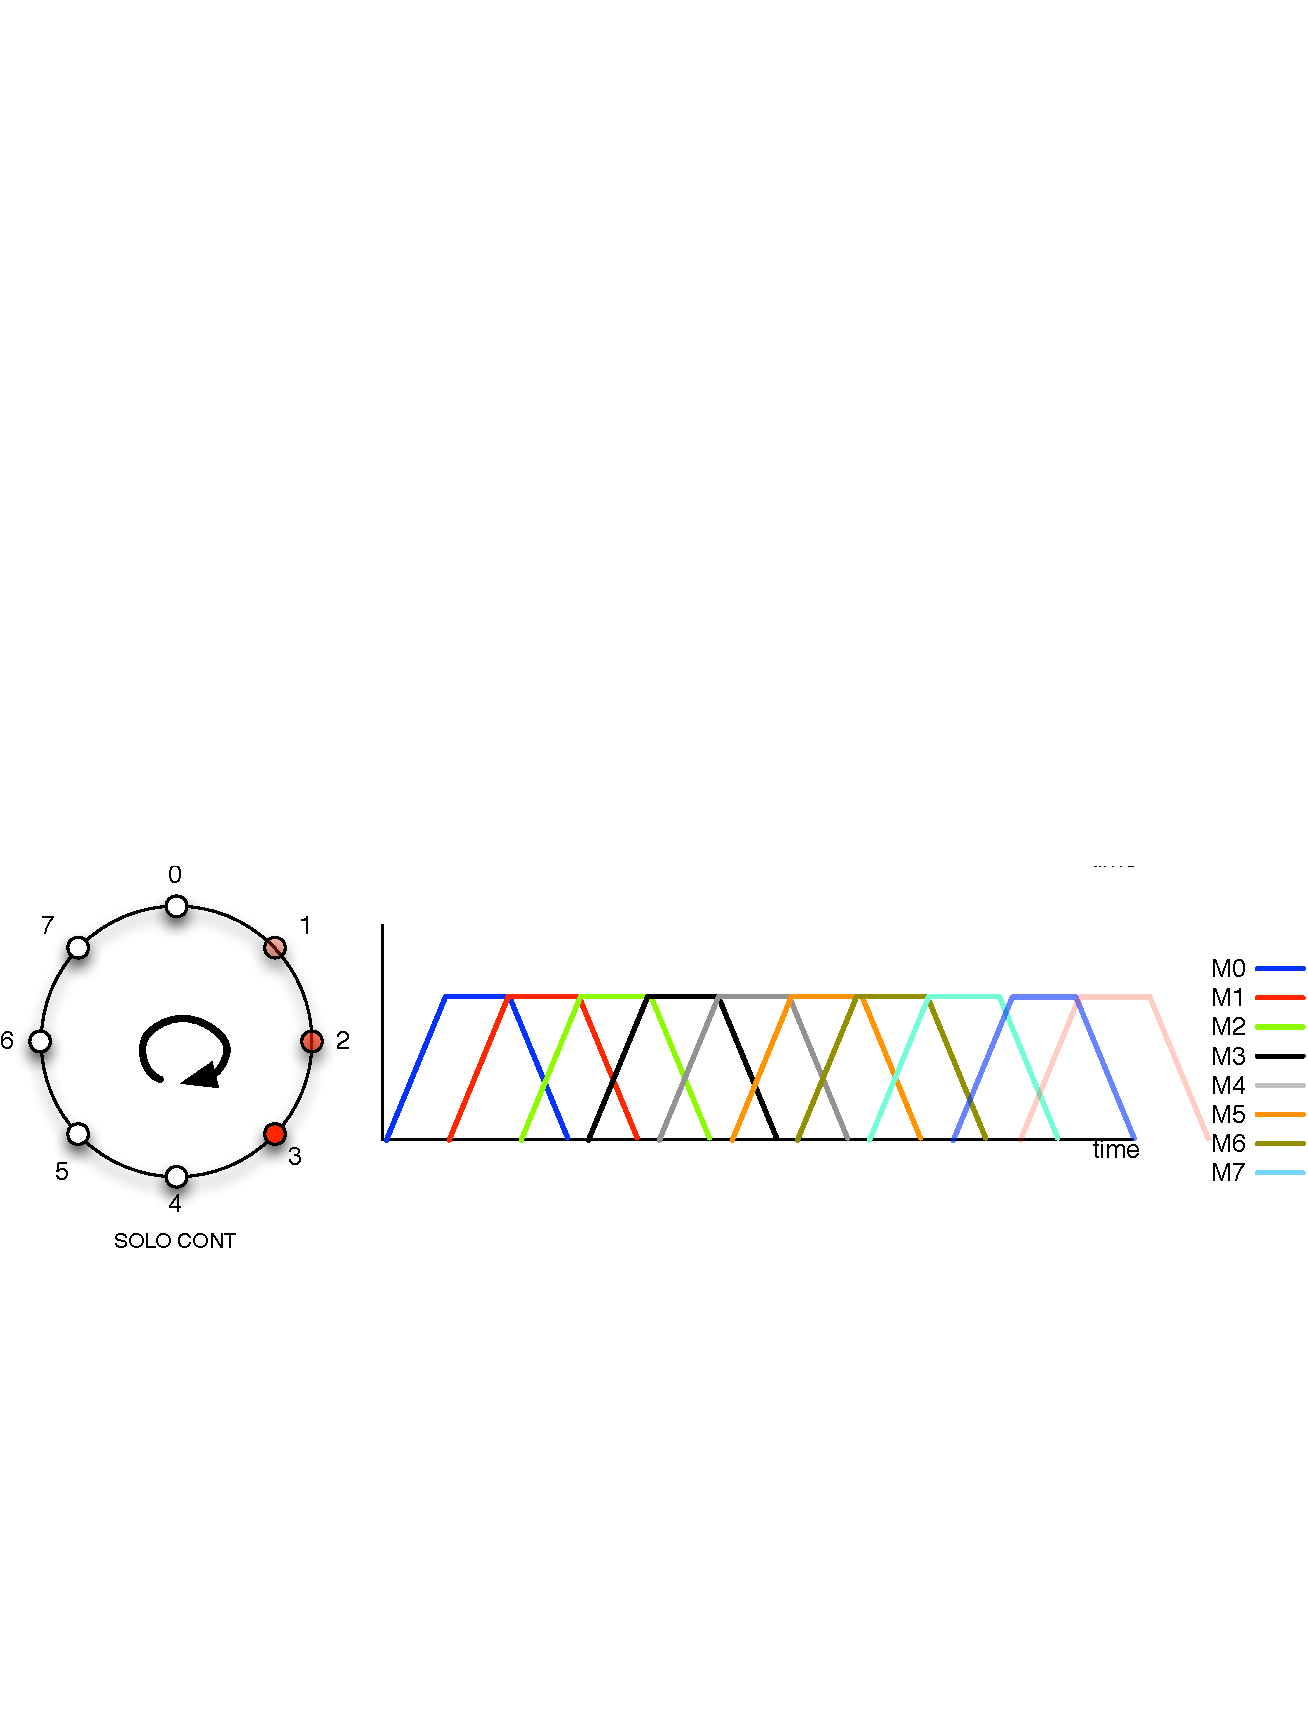
\includegraphics[width=1.0\textwidth]{pics/vibration_pattern_solo_cont}
\caption{The vibration pattern applied by the Tactile Belt to induce rotational movements in the blind user. The consequent vibrations motors are fired consecutively, starting from left for CW and right for CCW rotation.}
\label{fig:vibration_pattern_solo_cont}
\end{figure}

A special stop signal is applied to the belt when the user reaches the destination. Stop signal is implemented similar to \textbf{TWO TAPS} pattern except all the motors are activated instead of one


\subsection{Planning the Path of the User}

ROS provides an easy-to-use navigation stack for mobile robots. The input to the navigation stack is a map and a goal point and the output is a path and linear and angular velocities \emph{(v,w)} necessary to keep the robot on the course of the path. We assumed that the human is a non-holonomic robot with a circular footprint. The obstacle information is acquired from the laser scanner and the goal is provided in the sensor frame. Coupled with the Human Tracker, the 'robot' stays localized in the map and with respect to the path. The path is re-planned every second to deal with possible deviations. Next section is concerned with how the linear and angular velocities are converted to the vibration patterns.

\subsection{Velocity to Vibration Mapping}


Given a desired velocity that the 'robot' should execute, we first determine if a directional or rotational vibration pattern should be applied by the belt. If the linear velocity is dominant, then the human should walk towards that direction. If the angular velocity is dominant, the human should rotate around self. If both the linear and angular velocity is close to zero, the human should not move. To calculate which motion is appropriate, the 'robot' is simulated using Equation \ref{eq:motion_model}. If the distance the 'robot' took is larger than a threshold, then a directional vibration pattern is used. If it is less than the threshold, a rotational pattern is used. If both of the velocities are small enough, the no vibration is applied. 

When the human gets to the vicinity of the goal point, a special stop signal is applied to inform the person that the destination is reached. Stop signal is implemented similar to \textbf{TWO TAPS} pattern except all the motors are activated instead of one.

\subsection{Demonstration}

We demonstrated that our system can successfully guide a blindfolded person to a goal location in a room. Based on our evaluation results of vibration patterns, we used \textbf{CONT} for directional motions and \textbf{SOLO CONT} for rotational motions. The experimenter manually provided several goal poses using the GUI. Note that since the system is re-planning frequently, the planner is able to accommodate dynamic obstacles and compensate unpredictable motions of the person. The demonstration steps as well as their explanations are shown in Figure~\ref{fig:blindguidepics}.

\begin{figure*}[ht!]
\centering
%
        \subfigure[]{%
            \label{fig:blindguide1}
            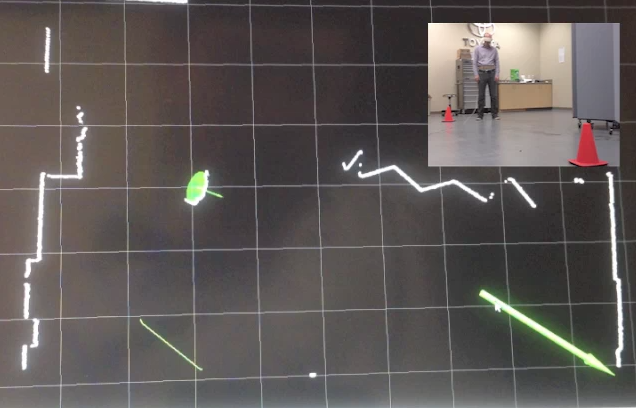
\includegraphics[width=0.46\columnwidth]{pics/blindguide1}
        }%
        \subfigure[]{%
           \label{fig:blindguide2}
           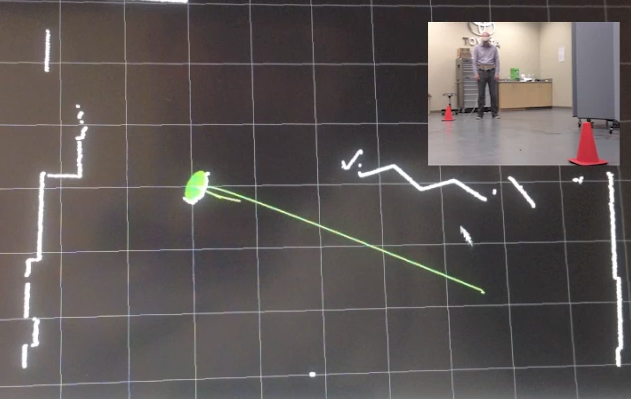
\includegraphics[width=0.46\columnwidth]{pics/blindguide2}
        }
        \subfigure[]{%
           \label{fig:blindguide3}
           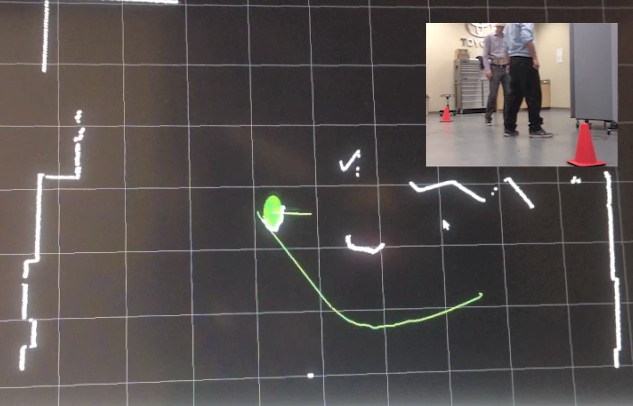
\includegraphics[width=0.46\columnwidth]{pics/blindguide3}
        }
\subfigure[]{%
           \label{fig:blindguide4}
           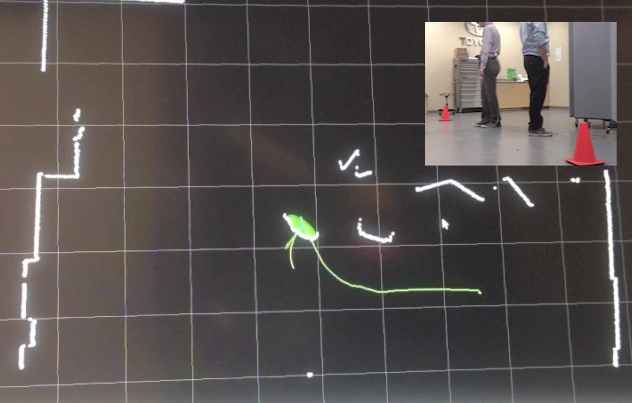
\includegraphics[width=0.46\columnwidth]{pics/blindguide4}
        }
\subfigure[]{%
           \label{fig:blindguide5}
           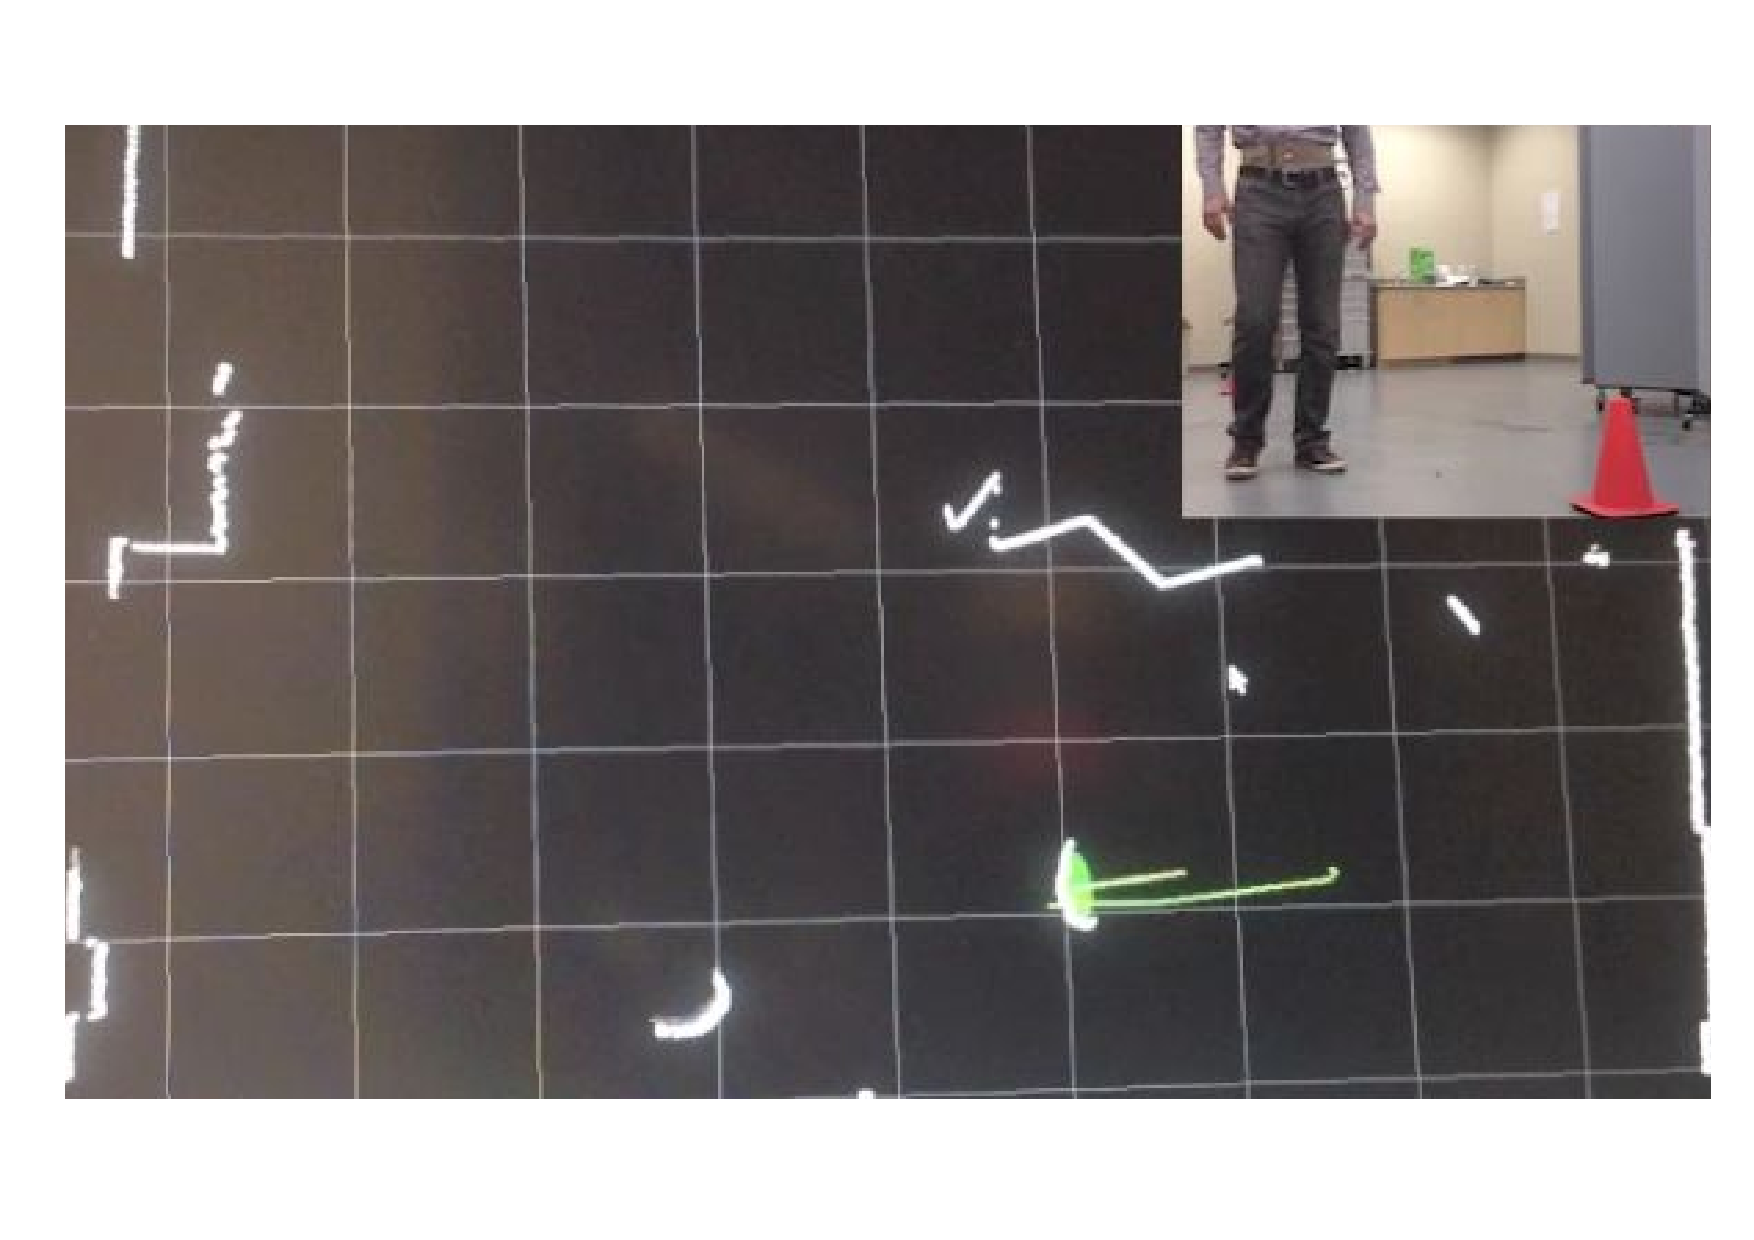
\includegraphics[width=0.46\columnwidth]{pics/blindguide5}
        }
\subfigure[]{%
           \label{fig:blindguide6}
           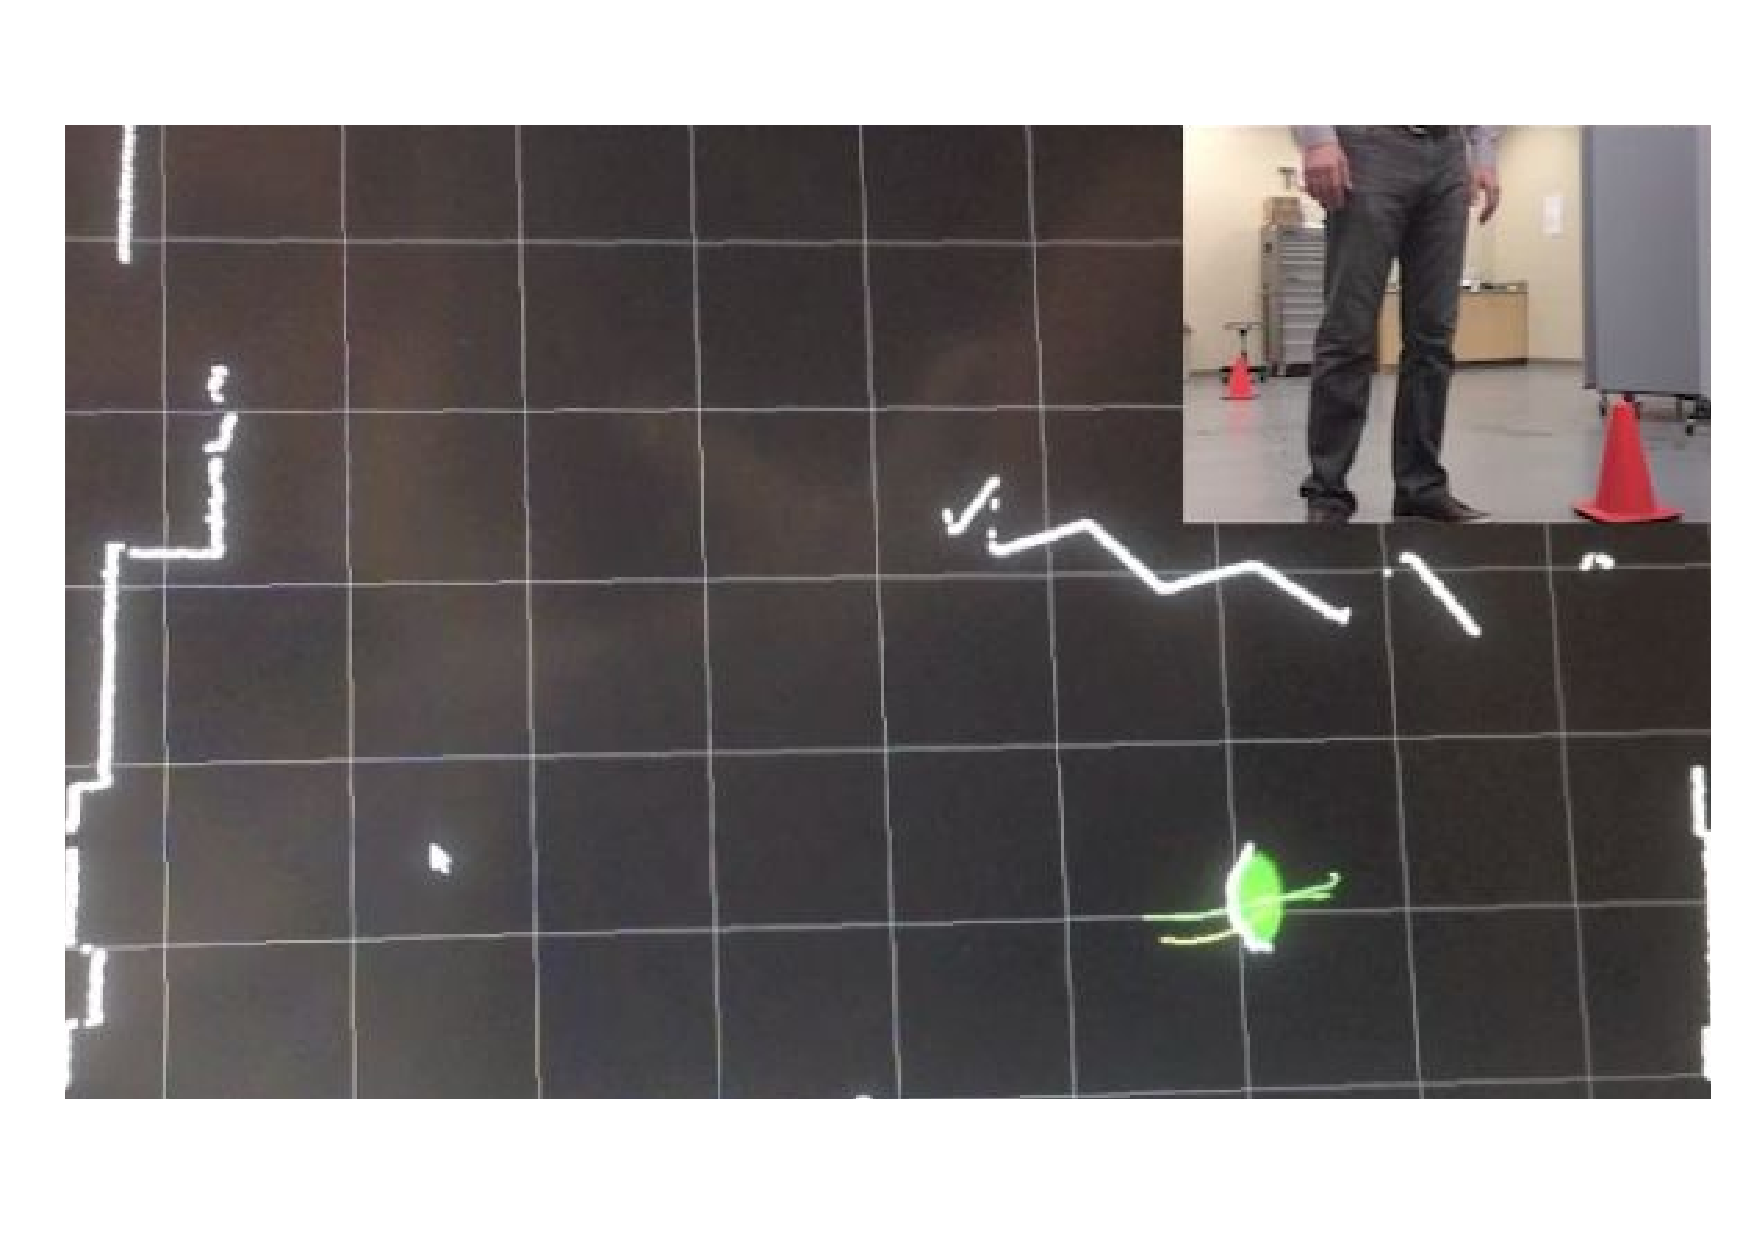
\includegraphics[width=0.46\columnwidth]{pics/blindguide6}
        }
    \caption{%
	Autonomous guiding of a blindfolded person using the tactile belt. a) The guidance starts. The user is blindfolded and is standing at the left of the screen. The human detection system detects him and places an ellipse marker with an arrow depicting his orientation. The operator gives a goal point by clicking on the screen. The goal point is the right traffic cone, and given by the big arrow. b) The system autonomously generates a path for the user. As seen in the picture the path is collision free. At this stage the belt begin to vibrate towards the front of the user. c) An unexpected obstacle (another person) appears and stops in front of the user. The system detects the other person as an obstacle, and reevaluates the path. A new path going around the obstacle is immediately calculated and sent to the user by the belt. d) The user receives a rotation vibration modality, and begins to turn towards the new path. And follows this path from now on. e) The obstacle leaves. The path is then reevaluated and changed. The user receives forward directional belt signal, and advances towards the goal. f) The person reaches to the vicinity of the goal and stop signal is applied.
     }%
   \label{fig:blindguidepics}
\end{figure*}

%%%%%%%%%%%%%%%%%%%%%%%%%%%%%%%%